\documentclass[tikz,border=2mm]{standalone}
\usepackage{emerald}
\usepackage[T1]{fontenc}
\usepackage{tikz}

\usetikzlibrary{positioning, matrix, arrows.meta,calc,decorations.pathmorphing}

\makeatletter

\pgfdeclaredecoration{penciline}{initial}{
    \state{initial}[width=+\pgfdecoratedinputsegmentremainingdistance,auto corner on length=1mm,]{
        \pgfpathcurveto%
        {% From
            \pgfqpoint{\pgfdecoratedinputsegmentremainingdistance}
                            {\pgfdecorationsegmentamplitude}
        }
        {%  Control 1
        \pgfmathparse{0.1*rand}
        \pgfpointadd{\pgfqpoint{\pgfdecoratedinputsegmentremainingdistance}{0pt}}
                        {\pgfqpoint{-\pgfdecorationsegmentaspect\pgfdecoratedinputsegmentremainingdistance}%
                                        {\pgfmathresult\pgfdecorationsegmentamplitude}
                        }
        }
        {%TO 
        \pgfpointadd{\pgfpointdecoratedinputsegmentlast}{\pgfpoint{1pt}{1pt}}
        }
    }
    \state{final}{}
}
\makeatother

\begin{document}\ECFJD

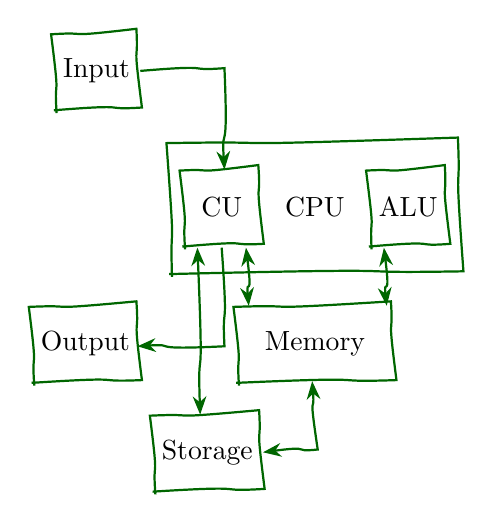
\begin{tikzpicture}[
    myline/.style={draw=green!40!black, thick, decoration=penciline, decorate},
    box/.style={myline, minimum height=1cm, minimum width=1cm, inner sep=.3333em}, >=Stealth]

    \matrix (CPU) [matrix of nodes, inner ysep=3mm, nodes=box, myline, column sep=1mm]
    {|(CU)|CU & |[draw=none]|CPU & |(ALU)| ALU \\};

    \node[box, above left=5mm of CPU] (input) {Input};
    \node[box, below left=5mm of CPU] (output) {Output};
    \node[box, at=(CPU|-output), minimum width=2cm] (memory) {Memory};
    \node[box, below left=5mm of memory, anchor=north] (storage) {Storage};
    \draw[<->, myline] (storage)-|(memory);
    \draw[->,myline] (input)-|(CU);
    \draw[->,myline] (CU)|-(output);
    \draw[<->, myline] ($(CU.south west)!.2!(CU.south east)$) coordinate (aux)--(aux|-storage.north);
    \draw[<->, myline] ($(CU.south west)!.8!(CU.south east)$) coordinate (aux)--(aux|-memory.north);
    \draw[<->, myline] ($(ALU.south west)!.2!(ALU.south east)$) coordinate (aux)--(aux|-memory.north);
\end{tikzpicture}
\end{document}
